\documentclass[spanish,10pt,a4paper]{article}
\usepackage[utf8]{inputenc}
\usepackage[T1]{fontenc}
\usepackage[left=2.00cm, right=2.00cm, top=2.00cm, bottom=2.00cm]{geometry}
\label{key}\usepackage{babel}
\usepackage{amssymb}
\usepackage{graphicx}
\usepackage{mathtools}
\usepackage{amsthm}
\usepackage{cite}
\usepackage{url}
\bibliographystyle{plain}
\begin{document}
	\title{Informe Del Proyecto De Programación Moogle!}
	\author{Roberto Manuel Martínez Nápoles}
	\date{Julio, 2023}
	\maketitle
	\begin{abstract}
		\center 
		1er Año de Ciencia de la Computación  
	\end{abstract}
	\begin{figure}[h]
	\center
	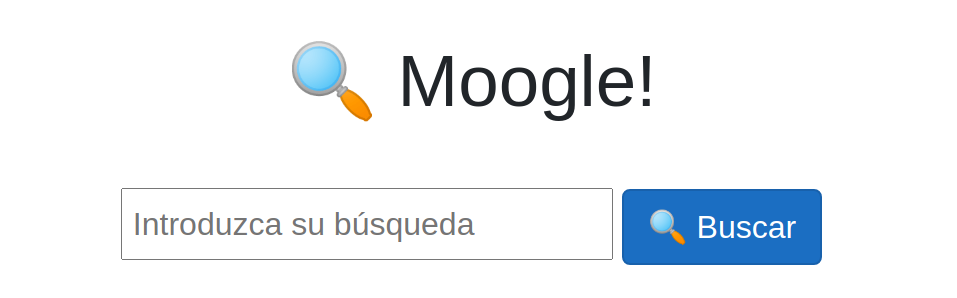
\includegraphics[width=12cm]{foto/moogle.png}
	\end{figure}
	
	\newpage
	
	
	\section{Introducción}\label{sec:intro}
	El proyecto consistía en crear una aplicación web de búsqueda matricial llamado Moogle!.  Esta aplicación buscará palabras o frases dentro de un contenedor que tiene una serie de documentos con extensión txt, y como resultado devolverá los documentos que contengan esas palabras o frases. 
	La aplicación  procesará los documentos antes de iniciar para calcular previamente una serie de valores necesarios e inprescindibles para la búsqueda. De esta tarea se encarga el método Matrix  de la clase moogle que ejecutará cuatro métodos de la clase TF-IDF-Matriz. Una clase que obtedrá una lista general de todas las palabras de los documentos, la cual transformará en una matriz de TF-IDF(Term Frecuency - Inverse Document Frecuency).
	Para la búsqueda realizada por un usuario (query) se dispone del método SimilitudDeCosenos de la clase moogle, el cual calculará un score por cada documento, donde ese score es la similitud que posee la query con un documento determinado. Y al final devolverá como resultado de la búsqueda los documentos relevantes para la query.
	
	
	
	\newpage
	\section{Utilización}\label{sec:utilización}
	Moogle! tiene una carpeta llamada Content la cual es donde están los documentos además de que se le puede agregar más contenidos. La carpeta MoogleEngine es la que contiene todas las clases del código que se ejecuta la aplicación cuando  está en funcionamiento. La carpeta MoogleServer es la que monta la red local donde funciona el Moogle!.
	
	Para usar el Moogle! solo tienes que entrar es su página web local y escribir una entrada y hacer click en el botón buscar y después de unos instantes se te mostrarán los documentos que coincidían con la búsqueda y una parte del texto del documento documento donde se encontró la coincidencia.
    
    \section{Funcionamiento}\label{sec:funcionamiento}
    La MoogleEngine es la que contiene las clases que estructuran el funcionamiento de la aplicación. La clase principal es moogle la cual 
    realiza la búsqueda usando métodos propios y de las demás clases auxiliares.
   
    Antes de ejecutarse la aplicación se ejecuta el método static void Matrix que crea el vocabulario de todas las palabras existentes en los documentos dentro de la carpeta Content y crean una matriz con el Tf-Idf de cada palabra en en cada documento el cual es el producto de dos medidas, frecuencia de término y frecuencia inversa de documento . Existen varias maneras de determinar el valor de ambas pero el Moogle! usa la manera normalizada, para evitar una predisposición hacia los documentos largos. Por ejemplo se divide la frecuencia bruta por la frecuncia máxima de algún término en el documento:
     \begin{equation}\label{eq:Tf}
    	        Tf(t,d) = f(t,d)/max{f(f,d): t \in d }    	                   
     \end{equation}
     
     La frecuencia inversa de documento es una medida de si el término es común o no, en la colección de documentos. Se obtiene dividiendo el total de documentos por el número de documentos que continen el término, y se toma el logaritmo de ese cociente \texttt{equation}:
     \begin{equation}\label{eq:Idf}
     	Idf(t, D) = log  |D|/|{d \in D: t \in d}|
     \end{equation}
     donde:
     \begin{itemize}
     	\item[*] D: es el número de documentos en la colección.
           \item[*]| {$d \in $ D : $ t \in $d}| : número de documentos donde aparece el término t. Si el término no está en la colección se producirá una división por cero. Por lo tanto es común ajustar esta fórmula a 1+|{$d \in $D : $t \in $d}|.
                              
     \end{itemize}
    
     Matemáticamente, la base de la función logaritmo no es importante y constituye un factor constante en el resultado final.
     
     Luego se calcula como \texttt{equation:}
     \begin{equation}\label{eq:TfIdf}
     	TfIdf(t,d,D) = Tf(t,d) * Idf(t,D)
     \end{equation}
     
     Un peso alto en Tf-Idf se alcanza con una elevada frecuencia de término(en el docummento dado) y una pequeña frecuencia de ocurrencia del término en la colección completa de documentos. Como el cociente dentro de la función logaritmo del Idf es siempre mayor o igual que 1, el valor del Idf (y del Tf-Idf) es mayor o igual que 0. Cuando un término aparece en muchos documentos, el cociente dentro del logaritmo se acerca a 1, ofreciendo de Idf y de Tf-Idf cercano a 0.
     
     
     Después de creada la matriz se le aplica una norma a la matriz lo que devuelve un vector (N) y se inicializa la aplicación y se introduce la entrada y después de que el usuario comienza la búsqueda se ejecuta el método query que convierte la query en vector de Tf-Idf y multiplica el vector por la matriz para obtener otro vector (R) y también se le aplica al vertorQuery una norma lo que devuelve un número (T) y después se crea un  vector (S) que es igual: \texttt{equation}
     \begin{equation}
     	vector (S) = vector (R)\ vector (N)*(T)
     \end{equation}
     
     Que el vector (S) seria el puntaje que se le asignan a cada documento. Después ordena lo ducumentos por puntaje de mayor a menor les se extrae la parte del texto que coincidió con la entrada del usuario y se devuelven todos los documentos que tuvieron coincidencias con la entrada.
      
      
     
     \newpage
     \tableofcontents
     
        	
\end{document}